\scanpage{144}
\mspage{93}

définit bien comme tantôt
\[
 F(w)=W'_w\longrightarrow\pi_0(w\backslash W'),
\]
il faut prouver que c'est bijectif. Or, $W'$ étant
\deleted{lisse} $\mathcal W_\infty$-lisse sur $W$, on sait que l'inclusion
$W'_w\hookrightarrow{}_{w}\backslash W'$ est dans $\mathcal W_\infty$, a fortiori
induit un iso pour les $\pi_0$.

Ceci posé, si \inserted{on a} une factorisation de $f^{\unsure{\leftarrow|*}}\colon$\deleted{\unsure{$V\to$}} $V'$
en $f=\pi\widetilde f$ ayant les propriétés a) b) de
la page précédente, on voit déjà que l'on a
\[
 f_!(e_V)\simeq\pi_!\bigl(\underbrace{\widetilde f_{\unsure{!}}(e_V)}_{\substack{\Vert\\e_{\widetilde V}\ \text{par b)}}}\bigr)\simeq\pi_!(e_{\widetilde V}),
\]
ce qui déjà détermine $\widetilde V$ à isom. \unsure{canonique|canoniques}
près (grâce à a) comme
\[
 \widetilde V\simeq V'_{/f_!(e_V)}\overset{\text{déf}}{=}\underline{\pi}_0(V'/V),
\]
et il ne doit pas être bien dur de se
convaincre que $\widetilde f$ n'est autre que la \deleted{\unsure{flèche}}
flèche canonique de la page 91.

\uline{Proposition 8} Pour qu'un objet $H$ de $U^\wedge$

\figure{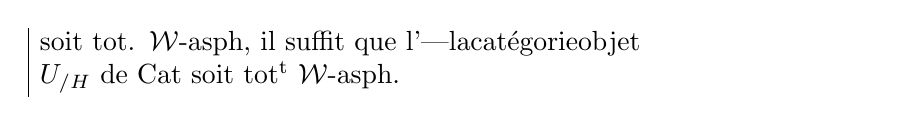
\begin{tikzpicture}
\node[anchor=north west,align=left,text width=.88\linewidth,inner xsep=4pt,inner ysep=1pt] (statement) at (0,0) {soit tot. $\mathcal W$-asph, il suffit que \unsure{l'|la}\deleted{catégorie}\inserted{objet}\\
$U_{/H}$ de $\mathrm{Cat}$ soit $\mathrm{tot}^{\mathrm t}$ $\mathcal W$-asph.};
\draw (statement.north west) -- (statement.south west);
\end{tikzpicture}}

% archive sheet number: 144
